\documentclass[conference]{IEEEtran}
\IEEEoverridecommandlockouts

\usepackage{cite}
\usepackage{amsmath,amssymb,amsfonts}
\usepackage{graphicx}
\usepackage{textcomp}
\usepackage{xcolor}
\usepackage{url}
\usepackage{hyperref}

% make sure captions are small font
\usepackage{subcaption}
\usepackage{caption}
\captionsetup{font=small}
\captionsetup[sub]{font=small}

\def\BibTeX{{\rm B\kern-.05em{\sc i\kern-.025em b}\kern-.08em
    T\kern-.1667em\lower.7ex\hbox{E}\kern-.125emX}}

\begin{document}

\title{Mixed-Integer Convex Programming for \\Motion Planning in Dual-Arm Manipulation}

\author{\IEEEauthorblockN{Phone Thiha Kyaw and Karyna Volokhatiuk}
\IEEEauthorblockA{\textit{University of Toronto Institute for Aerospace Studies} \\
Email: \{phone.thiha, karyna.volokhatiuk\}@robotics.utias.utoronto.ca}
}

\maketitle

\begin{abstract}
Motion planning for high-degree-of-freedom robotic manipulators is challenging due to complex constraints such as collision avoidance, kinematic limits, and trajectory smoothness.
%
In this project, we propose formulating the motion planning problem for dual-arm manipulation (14-DOF) as a convex optimization problem.
%
Specifically, we will leverage the recently studied Graph of Convex Sets (GCS) framework~\cite{marcucci2024shortest} to model motion planning as a compact mixed-integer optimization problem, similar to~\cite{marcucci2023motion}.
%
To evaluate its effectiveness, we will compare our approach against classical sampling-based motion planners from OMPL~\cite{sucan2012open}.
%
The proposed method will be implemented and tested in Drake~\cite{drake}, a widely used toolbox for modeling and simulating robotic systems.
\end{abstract}

\section{Introduction}

Motion planning is a fundamental problem in robotics that involves computing a feasible and efficient trajectory for a robot to move from an initial configuration to a goal configuration while satisfying various constraints\cite{lavalle2006planning}.
%
The problem becomes particularly challenging in high dimensional systems, which are generally known to be PSPACE-hard\cite{reif1979complexity}.

Classical approaches to motion planning rely heavily on sampling-based planners, such as Rapidly-exploring Random Trees (RRT)\cite{lavalle2001randomized} and Probabilistic Roadmaps (PRM)\cite{kavraki1996probabilistic}, due to their ability to efficiently explore high-dimensional spaces.
%
These planners have been widely adopted because they can handle complex environments without requiring an explicit representation of the free space.
%
However, when additional constraints such as kinodynamic feasibility, obstacle avoidance, or motion continuity are introduced, these methods struggle to produce high-quality, optimal trajectories.

Recent advances in optimization-based motion planning have tackled these limitations by formulating the problem as a compact mixed-integer convex program\cite{marcucci2023motion}.
%
One such approach, the Graph of Convex Sets (GCS) framework\cite{marcucci2024shortest}, enables the encoding of collision-avoidance constraints and system dynamics within a single convex optimization formulation.
%
By leveraging convex relaxations and mixed-integer programming, GCS provides a structured way to computing globally optimal trajectories while ensuring feasibility in constrained environments.

\begin{figure}[!t]
    \centering
    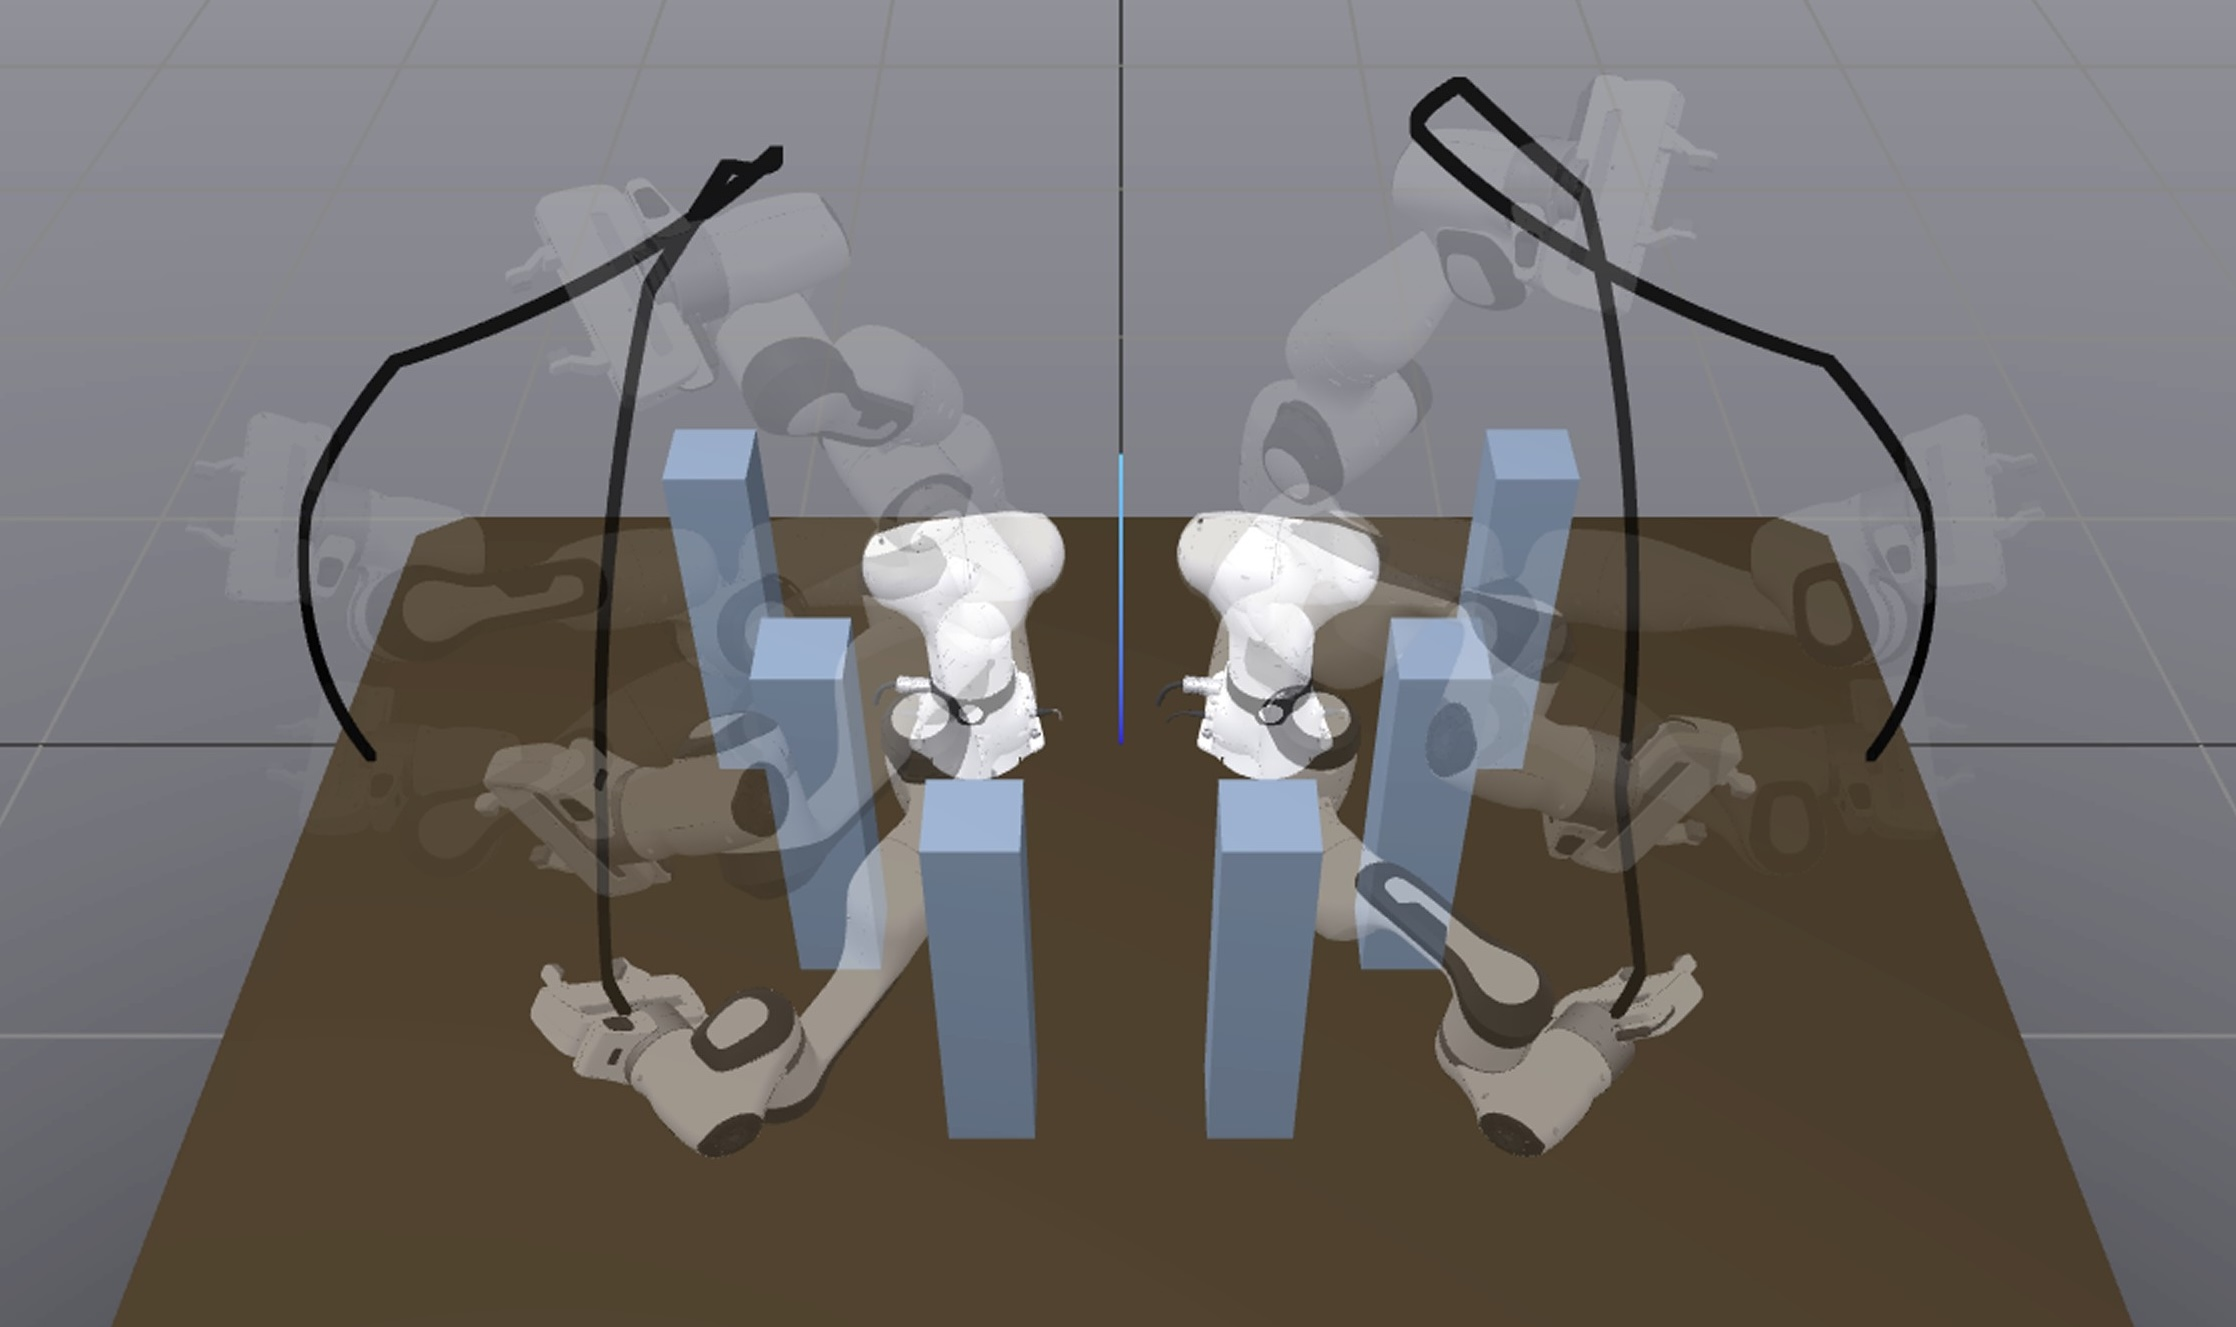
\includegraphics[width=0.99\linewidth]{figures/gcs_solution_trajectory_hd.jpg}
    \caption{A composite figure of two Franka Emika Panda robots executing a path found by our proposed convex optimization-based motion planning approach.}
    \label{fig:gcs_solution}
\end{figure}

\subsection{Contributions}
In this project, we explore the use of GCS framework for kinodynamic motion planning in dual-arm robotic manipulation (Figure~\ref{fig:gcs_solution}). Our key contributions are as follows:

\begin{itemize}
\item We formulate the problem of generating \textit{collision-free, kinodynamic motion plans} for a dual-arm manipulator as a mixed-integer convex program (MICP), following the approach in~\cite{marcucci2023motion}. However, unlike prior work, we investigate the scalability of the GCS framework in significantly higher-dimensional settings---specifically, an 18-degree-of-freedom (DOF) dual-arm system operating in a more complex, cluttered environment with narrow passages.
 
\item We conduct a comprehensive experimental study to evaluate the effectiveness of the optimization-based motion planning approach. Our experiments also include comparisons against recent sampling-based algorithms, analyzing critical performance metrics such as solution quality and computation time.
\end{itemize} 

This report is organized as follows: Section~\ref{sec:formulation} presents the problem formulation of our proposed approach. Section~\ref{sec:results} discusses and analyzes the results from our simulation studies. Finally, Section~\ref{sec:conclusion} concludes the report.
\section{Problem Formulation}\label{sec:formulation}

\subsection{Problem statement}
In this project, we formulate two problems. The simpler one involves using convex optimization to generate a trajectory of minimum Euclidean length between the initial and goal manipulator configurations. The more complex task extends this by also optimizing for trajectory duration and smoothness. The first solution will be fairly compared against sampling-based methods, which typically do not optimize for trajectory duration or smoothness. The second solution will be evaluated independently to analyze the effect of different weightings for the various optimization components: trajectory length, duration, and smoothness.

\subsection{IRIS}
First, it is important to note that the method we explore—Graph of Convex Sets (GCS)—requires as input a set of overlapping, convex, and collision-free regions (safe regions). To generate these regions, we use IRIS (Iterative Regional Inflation by Semidefinite Programming) \cite{iris}. While the construction of obstacle-free convex sets is itself an interesting topic, it is not the focus of this project; for more details, please refer to the original IRIS paper.

In brief, the user specifies a collision-free starting configuration for the robot, and the IRIS algorithm generates a convex polytope of valid configurations that includes this starting point. It is the user's responsibility to choose starting configurations that yield overlapping convex sets sufficient for constructing the desired path.

\subsection{Optimization problem: minimum-length trajectory}\label{sec:optimization_problem}

After constructing the safe regions using IRIS, we build a directed graph \( G = (V, E) \). Each vertex \( v \in V \) represents a collision-free convex region \(\mathcal{X}_v\), and a directed edge \( (u, v) \in E \) indicates that the corresponding regions \(\mathcal{X}_u\) and \(\mathcal{X}_v\) overlap (\(u, v \in V\)), allowing a transition from one to the other. Note that if \( (u, v) \in E \), then \( (v, u) \in E \). The length of each edge is variable and depends on two specific robot configurations, \(\mathbf{x}_u\) and \(\mathbf{x}_v\), chosen from the convex sets \(\mathcal{X}_u\) and \(\mathcal{X}_v\) that represent vertices \(U\) and \(V\) associated with the edge. The edge length is defined as the Euclidean distance between these two configurations: \( \| \mathbf{x}_v - \mathbf{x}_u \|_2 \). To enforce boundary conditions, two auxiliary vertices \( s, g \in V \) are introduced, corresponding to the start and goal configurations. For convenience, we set \(\mathcal{X}_s = \{\mathbf{x}_s\}\) and \(\mathcal{X}_g = \{\mathbf{x}_g\}\).

In this problem, we aim to find the minimum-length trajectory between configurations \(\mathbf{x}_s \in \mathcal{X}_s\) and \(\mathbf{x}_g \in \mathcal{X}_g\). For this, we can define a graph path \(p\) from vertex \(s\) to vertex \(g\) as a sequence of distinct vertices \((v_0, \ldots, v_K)\), where \(v_0 = s\) and \(v_K = g\). The corresponding sequence of edges is denoted by \(\mathcal{E}_p := \{ (v_0, v_1), \ldots, (v_{K-1}, v_K) \}\). We denote the set of all possible paths from \(s\) to \(g\) as \(\mathcal{P}\).

The optimization problem can then be formulated as:
\begin{equation}\label{eq:1}
\begin{aligned}
\text{minimize} \quad & \sum_{e = (u,v) \in \mathcal{E}_p} \left\| \mathbf{x}_v - \mathbf{x}_u \right\|_2 \\
\text{subject to} \quad 
& p \in \mathcal{P}, \\
& \mathbf{x}_u \in \mathcal{X}_u, \space \mathbf{x}_v \in \mathcal{X}_v,       & \forall u,v \in p, \\
& (\mathbf{x}_u, \mathbf{x}_v) \in \mathcal{X}_e, & \forall e = (u,v) \in \mathcal{E}_p.
\end{aligned}
\end{equation}

Here, the constraint \((\mathbf{x}_u, \mathbf{x}_v) \in \mathcal{X}_e\) is a convex constraint that couples the endpoints of edge \(e = (u, v)\). For the minimum Euclidean length trajectory problem, we can specify these constraints in the following way: for all edges $e = (u, v) \in \mathcal{E}$, we define $\mathcal{X}_e$ through the conditions \(\mathbf{x}_v \in \mathcal{X}_u \cap \mathcal{X}_v\) for \(\mathbf{x}_u \in \mathcal{X}_u\), \(\mathbf{x}_v \in \mathcal{X}_v\). This ensures that there is a collision-free path between two vertices.

At first glance, the problem in (\ref{eq:1}) may seem simple; however, its complexity lies in the need to not only minimize the total length of the trajectory but also determine which convex regions the path should traverse.

% brief GCS (nodes from IRIS and edges) --- note, we could have separate section for GCS too if it is too long, Mixed-Integer Formulation, final mathematical statement of our optimization problem

\subsection{Mixed-integer convex programming (MICP)}
\label{MICP_section}
The problem described in Section~\ref{sec:optimization_problem} can be formulated as mixed integer convex programming (MICP), a problem where certain decision variables are restricted to integers (usually binary), while others can be continuous. This combination leads to a non-convex optimization problem. Therefore, we follow the MICP formulation introduced by Marcucci et al. \cite{marcucci2024shortest}, which is based on the network-flow formulation and becomes convex after the relaxation step:
\begin{align}
\text{minimize} \quad & \sum_{e \in \mathcal{E}} \widetilde{\ell}_e(\mathbf{z}_e, \mathbf{z}'_e, y_e) \tag{2.1} \label{eq:2.1}\\
\text{subject to} \quad 
& \sum_{e \in \mathcal{E}_s^{\text{out}}} y_e = 1 \quad \sum_{e \in \mathcal{E}_g^{\text{in}}} y_e = 1 \tag{2.2} \\
& \sum_{e \in \mathcal{E}_v^{\text{out}}} y_e \le 1 \quad \forall v \in {V} \setminus \{s, g\} \tag{2.3} \\
& \sum_{e \in \mathcal{E}_v^{\text{in}}} (\mathbf{z}'_e, y_e) = \sum_{e \in \mathcal{E}_v^{\text{out}}} (\mathbf{z}_e, y_e) \quad \forall v \in {V} \setminus \{s, g\} \tag{2.4} \label{eq:2.4}\\
& (\mathbf{z}_e, y_e) \in \widetilde{\mathcal{X}}_u, \quad (\mathbf{z}'_e, y_e) \in \widetilde{\mathcal{X}}_v \quad \forall e = (u, v) \in \mathcal{E} \tag{2.5} \label{eq:2.5} \\
& y_e \in \{0, 1\} \quad \forall e \in \mathcal{E} \tag{2.6} \label{eq:2.6}
\end{align}

Here, \(y_e\) are the flows --- decision variables that define if edge \(e\) is traversed by the path (if \(y_e=1\), then is traversed). Other decision variables are $\mathbf{z}_e = y_e \mathbf{x}_u$ and $\mathbf{z}'_e = y_e \mathbf{x}_v$, where $e$ is an edge $e = (u,v)$; they represent the flow-weighted configuration of the vertex 
(either \(\mathbf{x}_u \in \mathcal{X}_u\), or \(\mathbf{x}_v \in \mathcal{X}_v\); \(u, v \in V\)) at one end of the edge.

The objective function (\ref{eq:2.1}) is a sum of perspective functions, which are based on the edge length. If we introduce a function \({\ell_e}\) as \(\| \mathbf{x}_v - \mathbf{x}_u \|_2\) when \((\mathbf{x}_u, \mathbf{x}_v) \in \mathcal{X}_e\) and \(\inf\) otherwise, the perspective function can be defined as:

\[
\tilde{\ell}_e(\mathbf{z}_e, \mathbf{z}'_e, y_e) =
\begin{cases}
\ell_e(\mathbf{x}_u, \mathbf{x}_v) y_e & \text{if } y_e > 0, \\

0, & \text{otherwise}.
\end{cases}
\]

The sets $\mathcal{E}_v^{\mathrm{in}} := \{(u, v) \in \mathcal{E}\}$ and $\mathcal{E}_v^{\mathrm{out}} := \{(v, u) \in \mathcal{E}\}$ represent the sets of edges incoming to and outgoing from vertex $v$, respectively. \(\tilde{\mathcal{X}}_u\) and \(\tilde{\mathcal{X}}_v\) are perspective cones of the convex sets $\mathcal{X}_u$ and $\mathcal{X}_v$, respectively. Constraints in \ref{eq:2.5} ensure that if $y_e = 1$ (edge $e$ is part of the selected path), then $z_e = x_u \in \mathcal{X}_u$ and $z_e' = x_v \in \mathcal{X}_v$; and if $y_e = 0$, then $z_e = z_e' = 0$. The purpose of these cones is to switch on/off vertex participation in the path without breaking convexity. Finally, \ref{eq:2.4} ensures flow conservation.

To achieve convexity, Marcucci et al.~\cite{marcucci2024shortest} relax the binary constraints in (\ref{eq:2.6}), allowing \( y_e \in [0, 1] \). This relaxed variable can be interpreted as the probability of edge \( e \) being included in the shortest path~\cite{marcucci2023motion}. The resulting formulation is a Second-Order Cone Program (SOCP).

Finally, to get an approximate solution, \cite{marcucci2023motion} proposes to round probabilities using a randomized depth-first search with backtracking (see Section 4.2 in \cite{marcucci2023motion} for details). After this step we can also calculate an (overestimated) optimality gap of the rounded solution: \( \delta_{\text{relax}} = (C_\text{round} - C_\text{relax}) / C_{\text{relax}} \).

\subsection{Extension of the optimization problem}
Due to space constraints and the increased complexity arising from optimizing not only Euclidean distance but also time and smoothness, we will briefly outline the core ideas behind the formulation proposed in \cite{marcucci2023motion}.

To enable this richer optimization, each trajectory is parameterized using two B\'ezier curves. Previously, a configuration variable \(\mathbf{x}_v \in \mathcal{X}_v\) was associated with each vertex \(v \in V\); now, each such variable corresponds to the set of control points for two B\'ezier curves. One curve represents the path (spatial component), while the other represents the time-scaling function.

The objective function is expressed as a weighted sum of three terms: the trajectory duration, its length, and the energy of the time derivative of the trajectory. The energy term promotes trajectory smoothness. Additional constraints are introduced to enforce a desired degree of differentiability, as well as to bound the total duration. Despite the increased number of constraints and the more complex objective, the Mixed-Integer Convex Programming (MICP) framework described in Section~\ref{MICP_section} remains applicable provided we suitably modify the edge cost function \({\ell_e}\) and incorporate the additional constraints into the graph edges. For a detailed discussion of the full formulation and solution approach, see~\cite{marcucci2023motion}.
\section{Simulation Results}\label{sec:results}

\subsection{Implementation details}

Our convex optimization-based motion planning approach is primarily built using Drake~\cite{drake}, a widely used toolbox for modeling, simulation and optimization of advanced robotic systems.
We used Drake's implementations of the GCS framework and IRIS to decompose the robot's free configuration space into convex regions.
Note that, to handle the mixed-integer programs generated by the GCS approach, we made use of the MOSEK optimization solver~\cite{mosek}, which supports large scale mixed-integer convex programs.

The robot platform used to validate our approach is a 14-degree-of-freedom dual-arm manipulator as shown in Figure~\ref{fig:simulation}.
The environment we designed resembles a cage, where the robot's task is to move from its initial configuratio---positioned between the first two rows of obstacles---to a goal configuration located between the last two rows of obstacles.
We purposefully constructed this setup to ensure that narrow passages appear in the high-dimensional configuration space of the robot, a known challenge for classical motion planners.
All aspects of the robot's geometry, kinematics and collisions were modeled using Drake's built in simulation and collision checking engines.

{\color{red} \textit{todo: add IRIS details here and the process about how we create and store convex regions}}

In addition to our approach, we use sampling-based motion planners from the Open Motion Planning Library (OMPL)~\cite{sucan2012open} as benchmarks for comparison.
All parameters related to these sampling-based planners were carefully reviewed and adjusted only as necessary to ensure a fair comparison; detailed configurations are omitted from this report.
Interested readers can find more information in our publicly available repository\footnote{\url{https://github.com/utiasSTARS/ece1505-w25-project}}.{\color{red}we should probably move this repo to our own}

\subsection{Comparison with multi-query planners}

% In this experiment, we compare our approach with multi-query sampling-based planners under conditions where precomputation is allowed.
% These planners, such as PRM~\cite{kavraki1996probabilistic} (and its lazy variants~\cite{bohlin2000path}) and Sparse Roadmap Spanners (SPARS)~\cite{dobson2014sparse}, precompute a roadmap (graph) before planning to speed up the solution search.
% We measure metrics such as the time required to find a solution (excluding precomputation), solution quality, and success rate.

\subsection{Comparison with anytime planners}

% We also compare our approach against anytime planners, which can asymptotically improve solution quality over time.
% Specifically, we consider RRT-Connect~\cite{kuffner2000rrt}, BIT*\cite{gammell2020batch}, AIT*\cite{strub2020adaptively}, and Greedy RRT*~\cite{kyaw2024greedy}.
% Here, we focus on how quickly each method finds a solution of comparable quality to ours, as well as its success rate.
\section{Conclusion and Discussion}\label{sec:conclusion}

In this project, we explored the use of the Graph of Convex Sets (GCS) framework for motion planning in high-dimensional dual-arm robotic manipulation tasks. By formulating the planning problem as a mixed-integer convex program (MICP), we demonstrated that feasible and near-optimal trajectories can be generated even in complex and cluttered environments.

While GCS requires greater setup effort and computational resources, it offers free certificates of optimality for complex motion planning tasks. This provides valuable insight into solution quality and serves as a theoretical benchmark for evaluating performance. We also show that careful selection of convex, collision-free regions has a significant impact on both the solution quality and runtime of the algorithm. This suggests promising directions for future work in exploring alternative approaches for handling an increasing number of convex sets. Overall, convex optimization-based motion planning proves to be a powerful tool for planning in complex environments---particularly when solution quality and theoretical guarantees are prioritized.

\bibliographystyle{IEEEtran}
\bibliography{IEEEabrv,main}

\end{document}
